\documentclass[dvipdfmx, titlepage, 11pt]{jsarticle}
\usepackage{tikz}
\usetikzlibrary{patterns}
\usetikzlibrary{intersections,calc,arrows}
\usepackage[top=20truemm,bottom=20truemm,left=15truemm,right=15truemm]{geometry}
\usepackage{enumerate}
\usepackage{multicol}
\usepackage{diagbox}
\usepackage{graphicx}

\makeatletter
\newcommand{\overarc}[1]{
  \setbox0\hbox{#1}%
  \ifdim\wd0<1em%
    \stackrel{\frown}{#1}%
  \else\ifdim\wd0<1.75em%
    \stackrel{\rotatebox{90}{\big)}}{#1}%
  \else\ifdim\wd0<2.5em%
    \stackrel{\rotatebox{90}{\Big)}}{#1}%
  \else\ifdim\wd0<3.25em%
    \stackrel{\rotatebox{90}{\bigg)}}{#1}%
  \else%
    \stackrel{%
      \rotatebox[origin=c]{90}{\mbox{%
        $\left.\vphantom{\rotatebox[origin=c]{90}{#1}}\right)$%
      }}%
    }{#1}%
  \fi\fi\fi\fi%
}
\makeatother

\newcommand{\ncircle}[1]{\textcircled{\scriptsize #1}}
\newcommand{\nbox}[1]{\fbox{\hspace{5pt} \textcircled{\scriptsize #1}\hspace{5pt} }}
\newcommand{\ebox}{\fbox{ \hspace{10pt} }}

\title{\Huge 数学}
\author{\LARGE 試験時間 : 50分}
\date{\LARGE 平成30年度筑波大附属高校\\[3cm] 大問は \fbox{\Large {\bf 1}} から \fbox{\Large {\bf 5}} まであります\\[0.5cm] 解答は解答用紙に記入して下さい}
\begin{document}
\maketitle

\newpage
\thispagestyle{empty}
 
\newpage

\newpage
\thispagestyle{empty}
 
\newpage

\setcounter{page}{1}
\noindent \fbox{\LARGE {\bf 1}}\hspace{10pt} 次の\textcircled{\scriptsize 1} 〜 \textcircled{\scriptsize 3}の \fbox{ \hspace{10pt} } にあてはまる数を求めなさい.
\begin{enumerate}[(1)]
\item $x+y=\sqrt{11}$,\ $x-y=\sqrt{3}$のとき, $x^{5}y^{5}=$ \nbox{1} である.\\[3cm]
\item 大小2個のさいころを同時に投げ, 出た目をそれぞれ$a,\ \ b$とするとき, 3本の直線$\displaystyle y = \frac{b}{a}x$,\ \ $\displaystyle y=\frac{a}{b}x$,\ \ $\displaystyle y = \frac{1}{2}x+1$が三角形をつくる確率は \nbox{2} である.\\[4cm]
  \begin{multicols}{2}
  \item 右の図のように, 傾きが負である直線が, 関数$y=x^{2}$のグラフおよび$x$軸と3点A,\ \ B,\ \ Cで交わっている. Bの$x$座標が1で, AB=BCであるとき, Cの$x$座標の値は \nbox{3} である.
    \begin{center}
      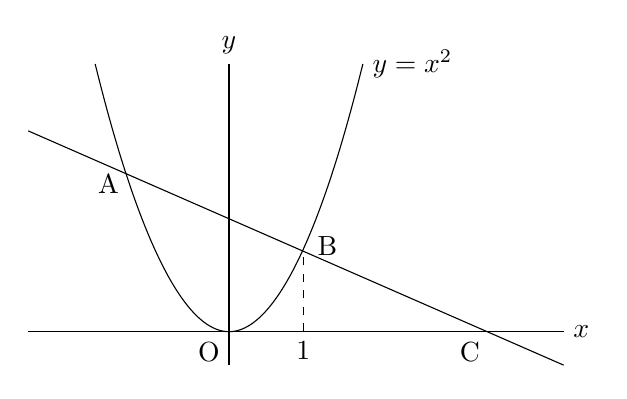
\begin{tikzpicture}[scale=0.85]
        \draw (-3,0)--(5,0) node[right] {$x$};
        \draw (0,-0.5) -- (0,4) node[above] {$y$};

        \draw[dashed] (1.11,0) node[below] {1}--(1.11,1.22);
        \node at (1.47,1.28) {B};
        \node at (-1.8,2.2) {A};
        \draw (-2,4) parabola bend (0,0) (2,4) node[right] {$y=x^{2}$};
        \draw (-3,3)--(5,-0.5);
        \node at (-0.3, -0.3) {O};
        \node at (3.6,-0.3) {C};
      \end{tikzpicture}
    \end{center}
  \end{multicols}
\end{enumerate}

\newpage

\noindent \fbox{\LARGE {\bf 2}}\hspace{10pt} 1日目は1円,\ \ 2日目は2円, $\cdots$ というように, 毎日1円ずつ金額を増やして貯金していき, 両替が可能な金額がたまり次第, 5円硬貨,\ 10円硬貨を用いて手持ちの硬貨をできるだけ少なくしていく.\\
例えば, 3日目には$1+2+3$で6円がたまるので, 手持ちの硬貨は5円硬貨1枚と1円硬貨1枚となる.\\
このとき, 次の \ncircle{4} 〜 \ncircle{6}の \ebox にあてはまる数を求めなさい.
\begin{enumerate}[(1)]
\item はじめて1円硬貨と5円硬貨がともに手持ちからなくなるのは4日目であるが, 2回目にそうなるのは \nbox{4} 日目である.\\[3cm]
\item 1日目から50日目までの間で, 1円硬貨と5円硬貨がともに手持ちからなくなる日は, 全部で \nbox{5} 回である.\\[3cm]
\item 123回目に1円硬貨と5円硬貨がともに手持ちからなくなるのは \nbox{6} 日目である.
\end{enumerate}

\newpage

\begin{multicols}{2}
  \noindent \fbox{\LARGE {\bf 3}}\hspace{10pt} 右の図のように, 長さ4cmの線分ABを直径とする円上に, AC=2cmとなる点Cをとり, BCを直径とする円と線分ABとの交点をDとする. また, 線分ACの中点をMとし, 線分BMと線分CD,\ \ 弧ACとの交点をそれぞれE,\ \ Fとする.\\
  このとき,\ \ 次の \ncircle{7} 〜 \ncircle{9} の \ebox にあてはまる数を求めなさい.
  \begin{center}
    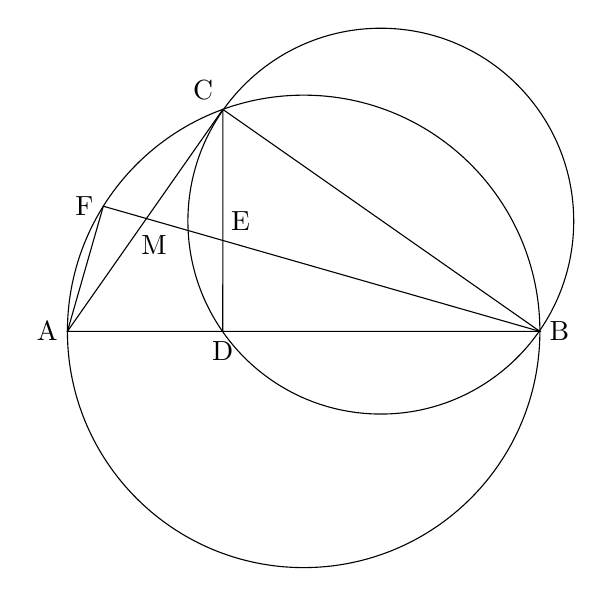
\begin{tikzpicture}
      \coordinate (A) at (-3,0);
      \coordinate (B) at (3,0);
      \coordinate (C) at (110:3);
      \coordinate (D) at ($(215:2.45)+(0.98,1.4)$);
      \coordinate (F) at (148:3);
      \draw (A)node[left]{A}--(B)node[right] {B}--(C)node[above left] {C}--cycle;
      \draw (A)--(F) node[left] {F}--(B);
      \draw (0,0) circle[radius=3];
      \draw (0.98,1.4) circle[radius=2.45];
      \draw (C)--(D) node[below] {D};
      \node at (-1.9,1.1) {M};
      \node at (-0.8,1.4) {E};
    \end{tikzpicture}
  \end{center}
\end{multicols}
\begin{enumerate}[(1)]
\item 線分CE,\ \ EDの長さの比を最も簡単な整数の比で表すと,
  \begin{center}
    CE : ED = \fbox{\hspace{5pt} \ncircle{7} - 1\hspace{5pt} } : \fbox{\hspace{5pt} \ncircle{7} - 2\hspace{5pt} }
  \end{center}
  である.\\[3cm]
\item 線分AFの長さは, \nbox{8} cmである.\\[3cm]
\item $\triangle$ADE,\ \ $\triangle$AFEの面積の比を最も簡単な整数の比で表すと,
  \begin{center}
    $\triangle$ADE : $\triangle$AFE = \fbox{\hspace{5pt} \ncircle{9} - 1\hspace{5pt} } : \fbox{\hspace{5pt} \ncircle{9} - 2\hspace{5pt} }
  \end{center}
  である.
\end{enumerate}

\newpage

\noindent \fbox{\LARGE {\bf 4}}\hspace{10pt} A地点からB地点に向かう長さ60mの一定速度で動く歩道(水平型エスカレーター, 以下「歩道」とする)がある. この歩道を利用する人は2列となり, 左の列は歩かない人が, 右の列は歩く人が利用している. AからBまでにかかる時間は, 歩かない人が75秒, 歩く人が30秒である.

このとき,\ \ 次の \ncircle{10} 〜 \ncircle{12} の \ebox \ にあてはまる数を求めなさい.

\begin{enumerate}[(1)]
\item 歩道が止まった場合, 右の列の人がAからBまで歩くのにかかる時間は \nbox{10} 秒かかる.\\[3cm]
\item 多くの人が2列に分かれて歩道を利用する. 9時ちょうど各列の先頭の人は同時にAを出発する. それぞれの列では人が等間隔に並ぶが, その間隔は右の列が左の列よりも2m長い. 9時5分に各列の人が同時にBに到達し, この5分間でBに到達した人数はどちらの列も等しかった.\\
  この5分間でBに到達した人数は全部で \nbox{11} 人である.\\
  また, Bにとうたつする人数が802人になる時刻は,
  \begin{center}
    9時 \fbox{\hspace{5pt} \ncircle{12} - 1\hspace{5pt} } 分 \fbox{\hspace{5pt} \ncircle{12} - 2\hspace{5pt} } 秒
  \end{center}
  である.
\end{enumerate}

\newpage
\begin{multicols}{2}
  \noindent \fbox{\LARGE {\bf 5}}\hspace{10pt} 1辺の長さが4cmの立方体ABCD-EFGHがある. 3点P,\ \ Q,\ \ Rそれぞれ頂点A,\ \ B,\ \ Gを同時に出発し, Pは辺AB上,\ \ Qは辺BC上,\ \ Rは辺GC上にそれぞれ毎秒1cmの速さで移動して, もう一方の頂点に到着したら停止する.\\
  このとき, 次の \ncircle{13} 〜 \ncircle{15} の \ebox にあてはまる数を求めなさい.

  \begin{center}
    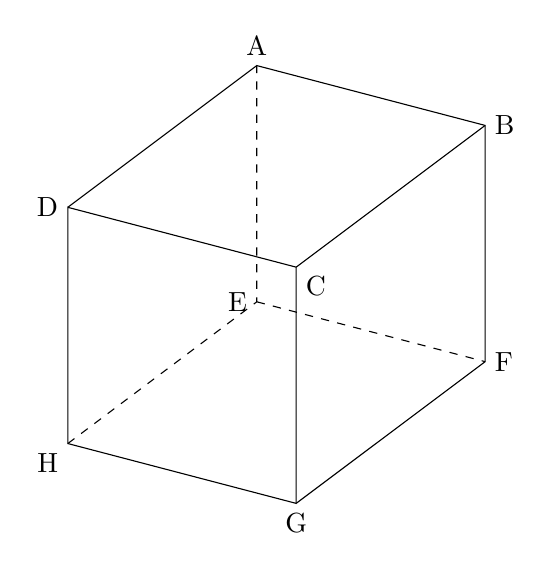
\begin{tikzpicture}
      \coordinate (H) at (0,0);
      \coordinate (D) at (0,3);
      \coordinate (G) at (2.9, -0.76);
      \coordinate (C) at (2.9,2.24);
      \draw (H)node[below left] {H}--(G)node[below] {G}--(C)node[below right] {C}--(D)node[left] {D}--cycle;
      \coordinate (E) at (2.4,1.8);
      \coordinate (F) at (5.3, 1.04);
      \coordinate (B) at (5.3, 4.04);
      \coordinate (A) at (2.4,4.8);
      \draw[dashed] (H)--(E)node[left] {E}--(A)node[above] {A};
      \draw[dashed] (E)--(F)node[right] {F};
      \draw (D)--(A)--(B)node[right] {B}--(F)--(G);
      \draw (B)--(C);
    \end{tikzpicture}
  \end{center}
\end{multicols}
\begin{enumerate}[(1)]
\item 3点P,\ \ Q,\ \ Rを通る平面でこの立方体を切断するときの切り口について考える.\\
  出発してから2秒経過したとき, 切り口の多角形の周の長さは \nbox{13} cmであり, 出発してから \nbox{14} 秒経過したとき, 点Eが切り口の多角形の頂点の1つとなる.\\[3cm]
\item 点Sは,\ \ P,\ \ Q,\ \ Rと同時に頂点Hを出発し, 毎秒2cmの速さでH $\to$ E $\to$ Hと辺HE上を往復する.\\
  出発する前2つの線分PRとQSは交わっているが, 出発後はじめて交わるのは, 出発してから \nbox{15} 秒経過したときである.
\end{enumerate}
\newpage
\thispagestyle{empty}
 
\newpage
\newpage
\thispagestyle{empty}
 
\newpage
\newpage
\thispagestyle{empty}
 
\newpage
\newpage
\thispagestyle{empty}
 
\newpage
\end{document}